\documentclass[11pt]{article}

\usepackage[utf8]{inputenc}
\usepackage[T1]{fontenc}
\usepackage{geometry}
\geometry{margin=1in}
\usepackage{times}
\usepackage{graphicx}
\usepackage{listings}
\usepackage{xcolor}
\usepackage{hyperref}
\usepackage{float}
\usepackage{microtype}

% Theo listing style
\definecolor{theokeyword}{HTML}{555555}
\definecolor{theostring}{HTML}{666666}
\definecolor{theotag}{HTML}{444488}

\lstdefinelanguage{theo}{
  morekeywords={ref, assert, suggest, question, thesis, evidence, counter, synthesis, tone},
  morestring=[b]",
  sensitive=true,
  literate=
    {==}{{\textcolor{theokeyword}{==}}}2
    {>}{{\textcolor{theokeyword}{>}}}1
    {>>}{{\textcolor{theokeyword}{>>}}}2
    {\#}{{\textcolor{theotag}{\#}}}1
    {@}{{\textcolor{theokeyword}{@}}}1,
}

\lstset{
  language=theo,
  basicstyle=\ttfamily\footnotesize,
  keywordstyle=\color{theokeyword},
  stringstyle=\color{theostring},
  frame=single,
  rulecolor=\color{gray!40},
  framesep=4pt,
  xleftmargin=6pt,
  xrightmargin=6pt,
  breaklines=true,
  columns=fullflexible,
  keepspaces=true,
  aboveskip=10pt,
  belowskip=10pt,
  tabsize=3,
}

\title{The Residue of Making}

\author{
  Mateo Larrea Ferro\\
  \textit{Stanford University}\\
  \texttt{mlarreaf@stanford.edu}
}

\date{}

\begin{document}
\maketitle

\begin{figure}[h]
  \centering
  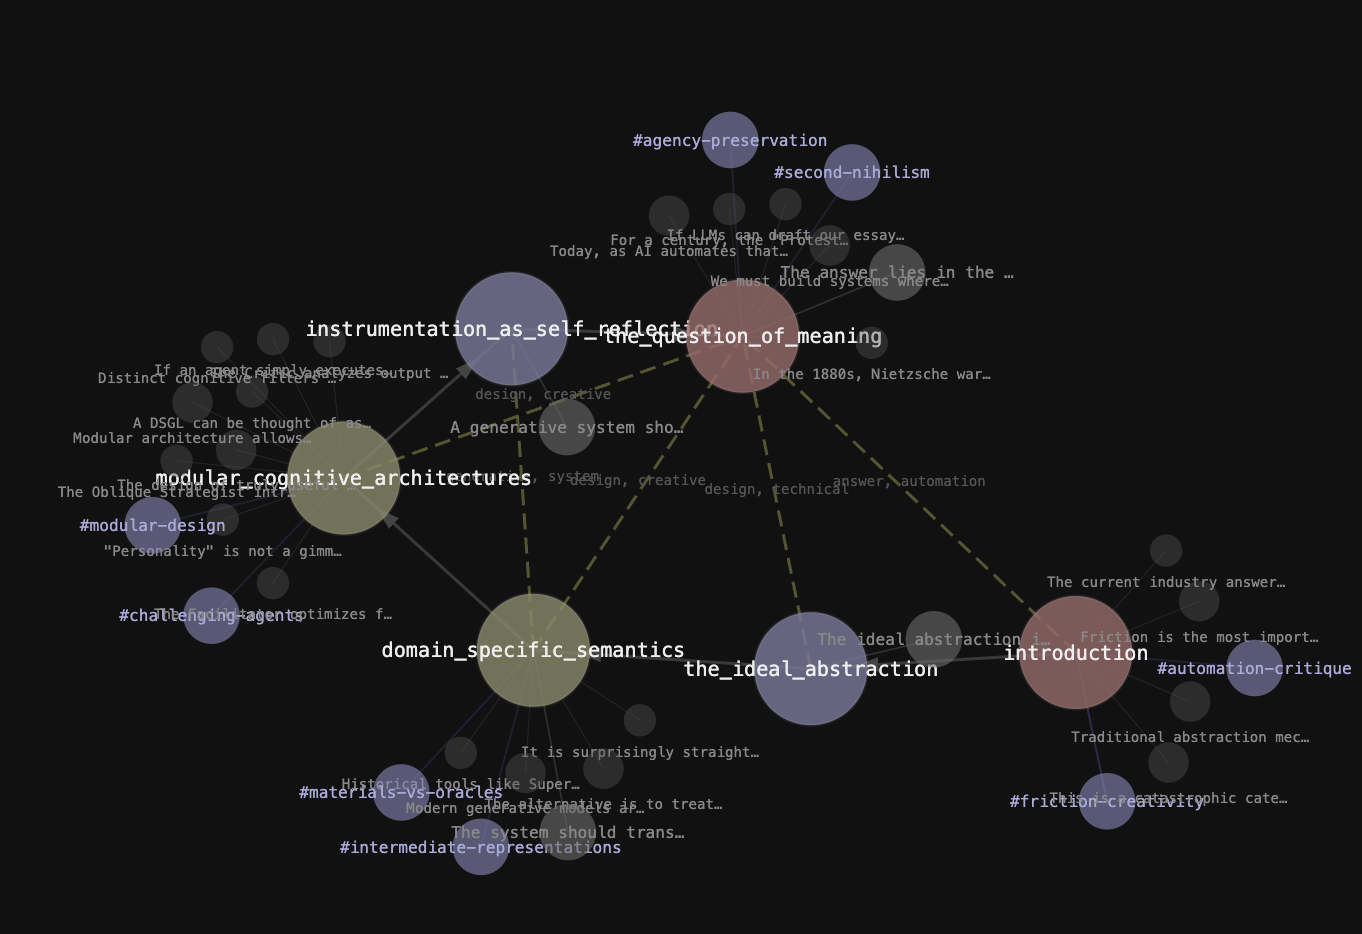
\includegraphics[width=0.585\textwidth]{Graph.png}
  \caption{A structural view of an essay authored with Theo, an early prototype of a Domain-Specific Generative Language. Sections appear as nodes colored by rhetoric mode; claims with shared tags produce cross-section edges.}
  \label{fig:graph}
\end{figure}

\section{Introduction}

A great portion of what we produce with generative Artificial Intelligence (AI) happens in a single exchange. A user writes a natural-language prompt, and the model returns a finished artifact. Suno\footnote{\url{https://suno.com}}, an AI music company, generates full songs---vocals, instrumentation, production---from a text description. ChatGPT produces polished essays from one-line instructions. Midjourney for image, Sora for video, and so on. In each case, the entire creative process collapses into one function call: intent in, artifact out. This paper calls it the \emph{oracle model}.

For many applications, this is perfectly fine. Not every piece of generated content requires human agency in its production. Drafting boilerplate code, summarizing documents, producing marketing copy at scale---these are tasks where the oracle model is efficient and often sufficient. In such contexts, the relevant measure is output quality relative to cost, and generative AI excels. This is the domain of \emph{content generation}: a world optimized for volume and speed, where the process of making is incidental overhead to be minimized.

But there is an overwhelming pressure to apply these same tools to creative tasks---writing, composing, designing---where the act of making is not incidental overhead but the core of the practice. For many practitioners, it is through engaging in the creative process that they develop introspection, refine their thinking, and find a sense of purpose. The accumulation of decisions---structural, aesthetic, rhetorical---is not a cost to be eliminated but the activity through which the work acquires meaning for the person doing it. When the tool absorbs the process, it does not just produce the artifact faster; it removes the activity that gave the artifact meaning to the maker.

This is not the first time a technology has moved practitioners up the ladder of abstraction. Programming languages evolved from machine code to assembly to high-level languages, each step trading direct control for expressive power. The recording industry moved from live performance to multitrack tape to digital production, each transition reshaping what it meant to ``make'' music. In each case, the community had to negotiate which parts of the process were worth preserving and which could be safely delegated to the machine. This paper asks a version of that same question for the age of generative AI: \emph{Is it still worth doing creative tasks as a human in a world where computers can produce similar results effortlessly?}

This paper argues yes---not sentimentally, but structurally. It examines why the creative process matters beyond its output, what the programming languages tradition reveals about the role of notation and agency in creative practice, and what properties a different kind of tool would need to have. It closes with Theo, a Domain-Specific Generative Language for essay composition, as an illustration of the kind of system that could preserve human agency within generative workflows.

\section{Why the Process Matters}

The introduction drew a line between content generation, where the oracle model is efficient and sufficient, and creative practice, where something essential is lost. But what, exactly, is lost? Not the artifact---generative models produce competent artifacts. What is lost is the process through which the artifact comes into being. And in creative work, that process is not overhead. It is constitutive.

Consider what happens when a composer writes a piece of music. The composer does not begin with a finished product in mind and then transcribe it. The process is recursive: an initial idea generates material, the material resists or suggests, and the composer responds. Harmonic rules constrain the space of possibilities, and within those constraints, unexpected combinations emerge. The composer discovers the piece through the act of making it. The final score is not just a product but a record of decisions, and those decisions are where the composer's relationship to the work resides.

The same holds for writing. A writer working through an argument does not simply externalize a pre-formed thought. The act of structuring claims, weighing evidence, confronting counter-arguments, choosing rhetorical emphasis: these are not mechanical steps that precede the ``real'' work. They \emph{are} the work. The essay that results is shaped by every commitment the writer made along the way. Remove those commitments, and what remains is text, but not authorship.

This is not a sentimental claim about the value of effort. It is a structural observation about what creative practice consists of. The productive friction between a practitioner's intent and a medium's constraints is the mechanism by which ideas are refined, by which the practitioner develops expertise, and by which the resulting artifact acquires the specificity that distinguishes it from a generic response to a generic prompt. When a tool eliminates this friction entirely, it does not merely speed up the process. It removes the process. And the process was the point.

\section{Editorial Control Is Not Authorial Control}

The standard response to this concern is that generative AI does not eliminate iteration. Users can refine: ``make it more formal,'' ``add a bridge in B minor,'' ``make the second paragraph more concise.'' The interface allows progressive adjustment, suggesting that the practitioner retains control over the result.

But there is a categorical difference between two kinds of control. When a programmer uses a type system to constrain the space of valid programs, they are making structural decisions that shape the artifact from within. The constraints are productive: they force the programmer to think about representation, about invariants, about the relationships between components. The resulting program reflects those decisions at every level.

When a user asks ChatGPT to ``make it shorter,'' they are adjusting surface features of an artifact whose structure was determined entirely by the model. The user did not choose the rhetorical strategy, the argumentative structure, the epistemic commitments, or the logical organization. The user is editing a finished product. This is editorial control: the ability to accept, reject, or modify an artifact that someone (or something) else has already constructed. It is not authorial control: the activity of making the structural decisions that constitute the work in the first place.

The distinction matters because the two activities produce fundamentally different relationships between the practitioner and the artifact. An author who has wrestled with the structure of an argument understands why it takes the form it does. An editor who has adjusted the surface of a generated argument may approve of the result without understanding, or having shaped, its internal logic. Both may produce competent text. Only one has engaged in the activity that constitutes writing.

\section{What the Programming Languages Tradition Reveals}

The introduction noted that generative AI is not the first technology to move practitioners up the ladder of abstraction. The programming languages community has studied this dynamic---the relationship between notation, thought, and agency---for decades, and its insights illuminate what the oracle model has displaced.

Iverson's ``Notation as a Tool of Thought''~\cite{iverson1980} established that the structure of a language determines the cognitive operations available to its users. A notation is not a passive recording device. It shapes what practitioners can think and do within a domain. The choice of primitives, the rules of composition, the constraints on valid expressions: these are not incidental features of a language. They define the space of possibilities available to the practitioner.

Creative coding extended this insight into artistic practice. Csound~\cite{vercoe1986} gave composers a language for defining instruments as mathematical expressions and scores as sequences of events. Processing~\cite{reas2007} gave visual artists a language for generating images and animations through code. In both cases, the formal language gave the practitioner direct access to the structural decisions that shape the work: which oscillator, what frame rate, how to compose two visual elements. The language amplified capability without hiding process. The practitioner learned to think in the medium's terms, and that fluency was itself a form of expertise.

Hudak~\cite{hudak1996} showed that restricting a language to a specific domain paradoxically expands its effective power, because the primitives align with the domain's natural abstractions. A domain-specific language sacrifices generality for expressiveness, making certain operations natural and others impossible. The restrictions become productive precisely because they foreground the choices that matter within the domain and eliminate the noise of irrelevant possibilities.

Prompt-based generative tools do the opposite. They remove the language entirely. There is no notation, no set of domain-specific primitives, no compositional structure that the practitioner can learn, internalize, and reason about. The user describes an intention in natural language, and the model returns a result. The intermediate layer, the formal system that mediates between intention and result, that provides a site for expertise and a locus of structural decision-making, disappears. What remains is input and output, with nothing in between.

This is the core of the problem. Generative models have eliminated the intermediate representations where creative decisions are made. The representations exist internally (attention patterns, latent embeddings, chain-of-thought traces), but none of them are accessible to the user. There is no user-facing structure between intent and artifact. And it is precisely in that intermediate space that art-making, as an activity, resides.

\section{Pinning Down the Contours}

If this analysis is correct, then the problem has several properties worth stating explicitly.

First, the problem is \textbf{not about quality}. The outputs of current generative models are often impressive. Suno produces songs that sound professionally produced. ChatGPT produces essays that are grammatically correct and logically structured. Quality is beside the point. The question is whether the practitioner had a meaningful role in producing it.

Second, the problem is \textbf{phenomenological}. It concerns what it is like to engage in a creative activity, not what the activity produces. Two artifacts may be identical: one made through a sustained process of decision-making, the other generated from a single prompt. The artifacts are the same. The experiences of the people who produced them are not. If the experience of making is part of why art-making matters (to the maker, to the development of expertise, to the cultivation of a practice), then the single-prompt workflow represents a loss even when the output is good.

Third, the problem is \textbf{about intermediate representations}. In a traditional compilation pipeline, intermediate representations serve as points of inspection and intervention. A programmer can examine the abstract syntax tree, reason about the type-checked representation, inspect the optimized output. Each stage is a locus of understanding and control. Prompt-based generation exposes exactly one representation: the final output. There is nothing the practitioner can inspect or modify structurally.

Fourth, the problem is \textbf{domain-general}. Although this paper has drawn examples from music, writing, and visual art, the underlying structure is the same across creative domains. Wherever a generative model collapses the space between intention and artifact, the same displacement occurs: the decisions that constitute the practice are absorbed by the model, and the practitioner is left with only the endpoints.

A notation that restores the intermediate layer would need to satisfy several constraints at once. It must be \emph{generatable}: an LLM must be able to produce it from natural-language input, so that the practitioner is not required to learn the notation before benefiting from it. It must be \emph{inspectable}: a domain practitioner must be able to read it and understand the structural decisions it encodes. It must be \emph{predictably editable}: local changes should produce local effects in the rendered output. It must be \emph{semantically rich}: its primitives should correspond to the meaningful abstractions of the domain (sections, claims, arguments, rhetoric modes), not to tokens or word counts. And it must be \emph{composable}: structural elements should combine in principled ways that support reasoning about the whole.

These constraints pull against each other. Generatability favors simplicity; semantic richness favors complexity. Inspectability requires surface-level readability; composability requires formal structure that may resist it. The right trade-offs are likely domain-dependent, and different creative domains may require fundamentally different notations. This paper does not resolve these tensions. It identifies them as the contours of a problem that matters: how to build tools for art-making that preserve the making. The answer to the question posed at the outset---whether it is still worth doing creative tasks as a human in a world where machines can produce similar results---is yes, but only if the tools we build leave room for the doing.

\begin{figure}[t]
  \centering
  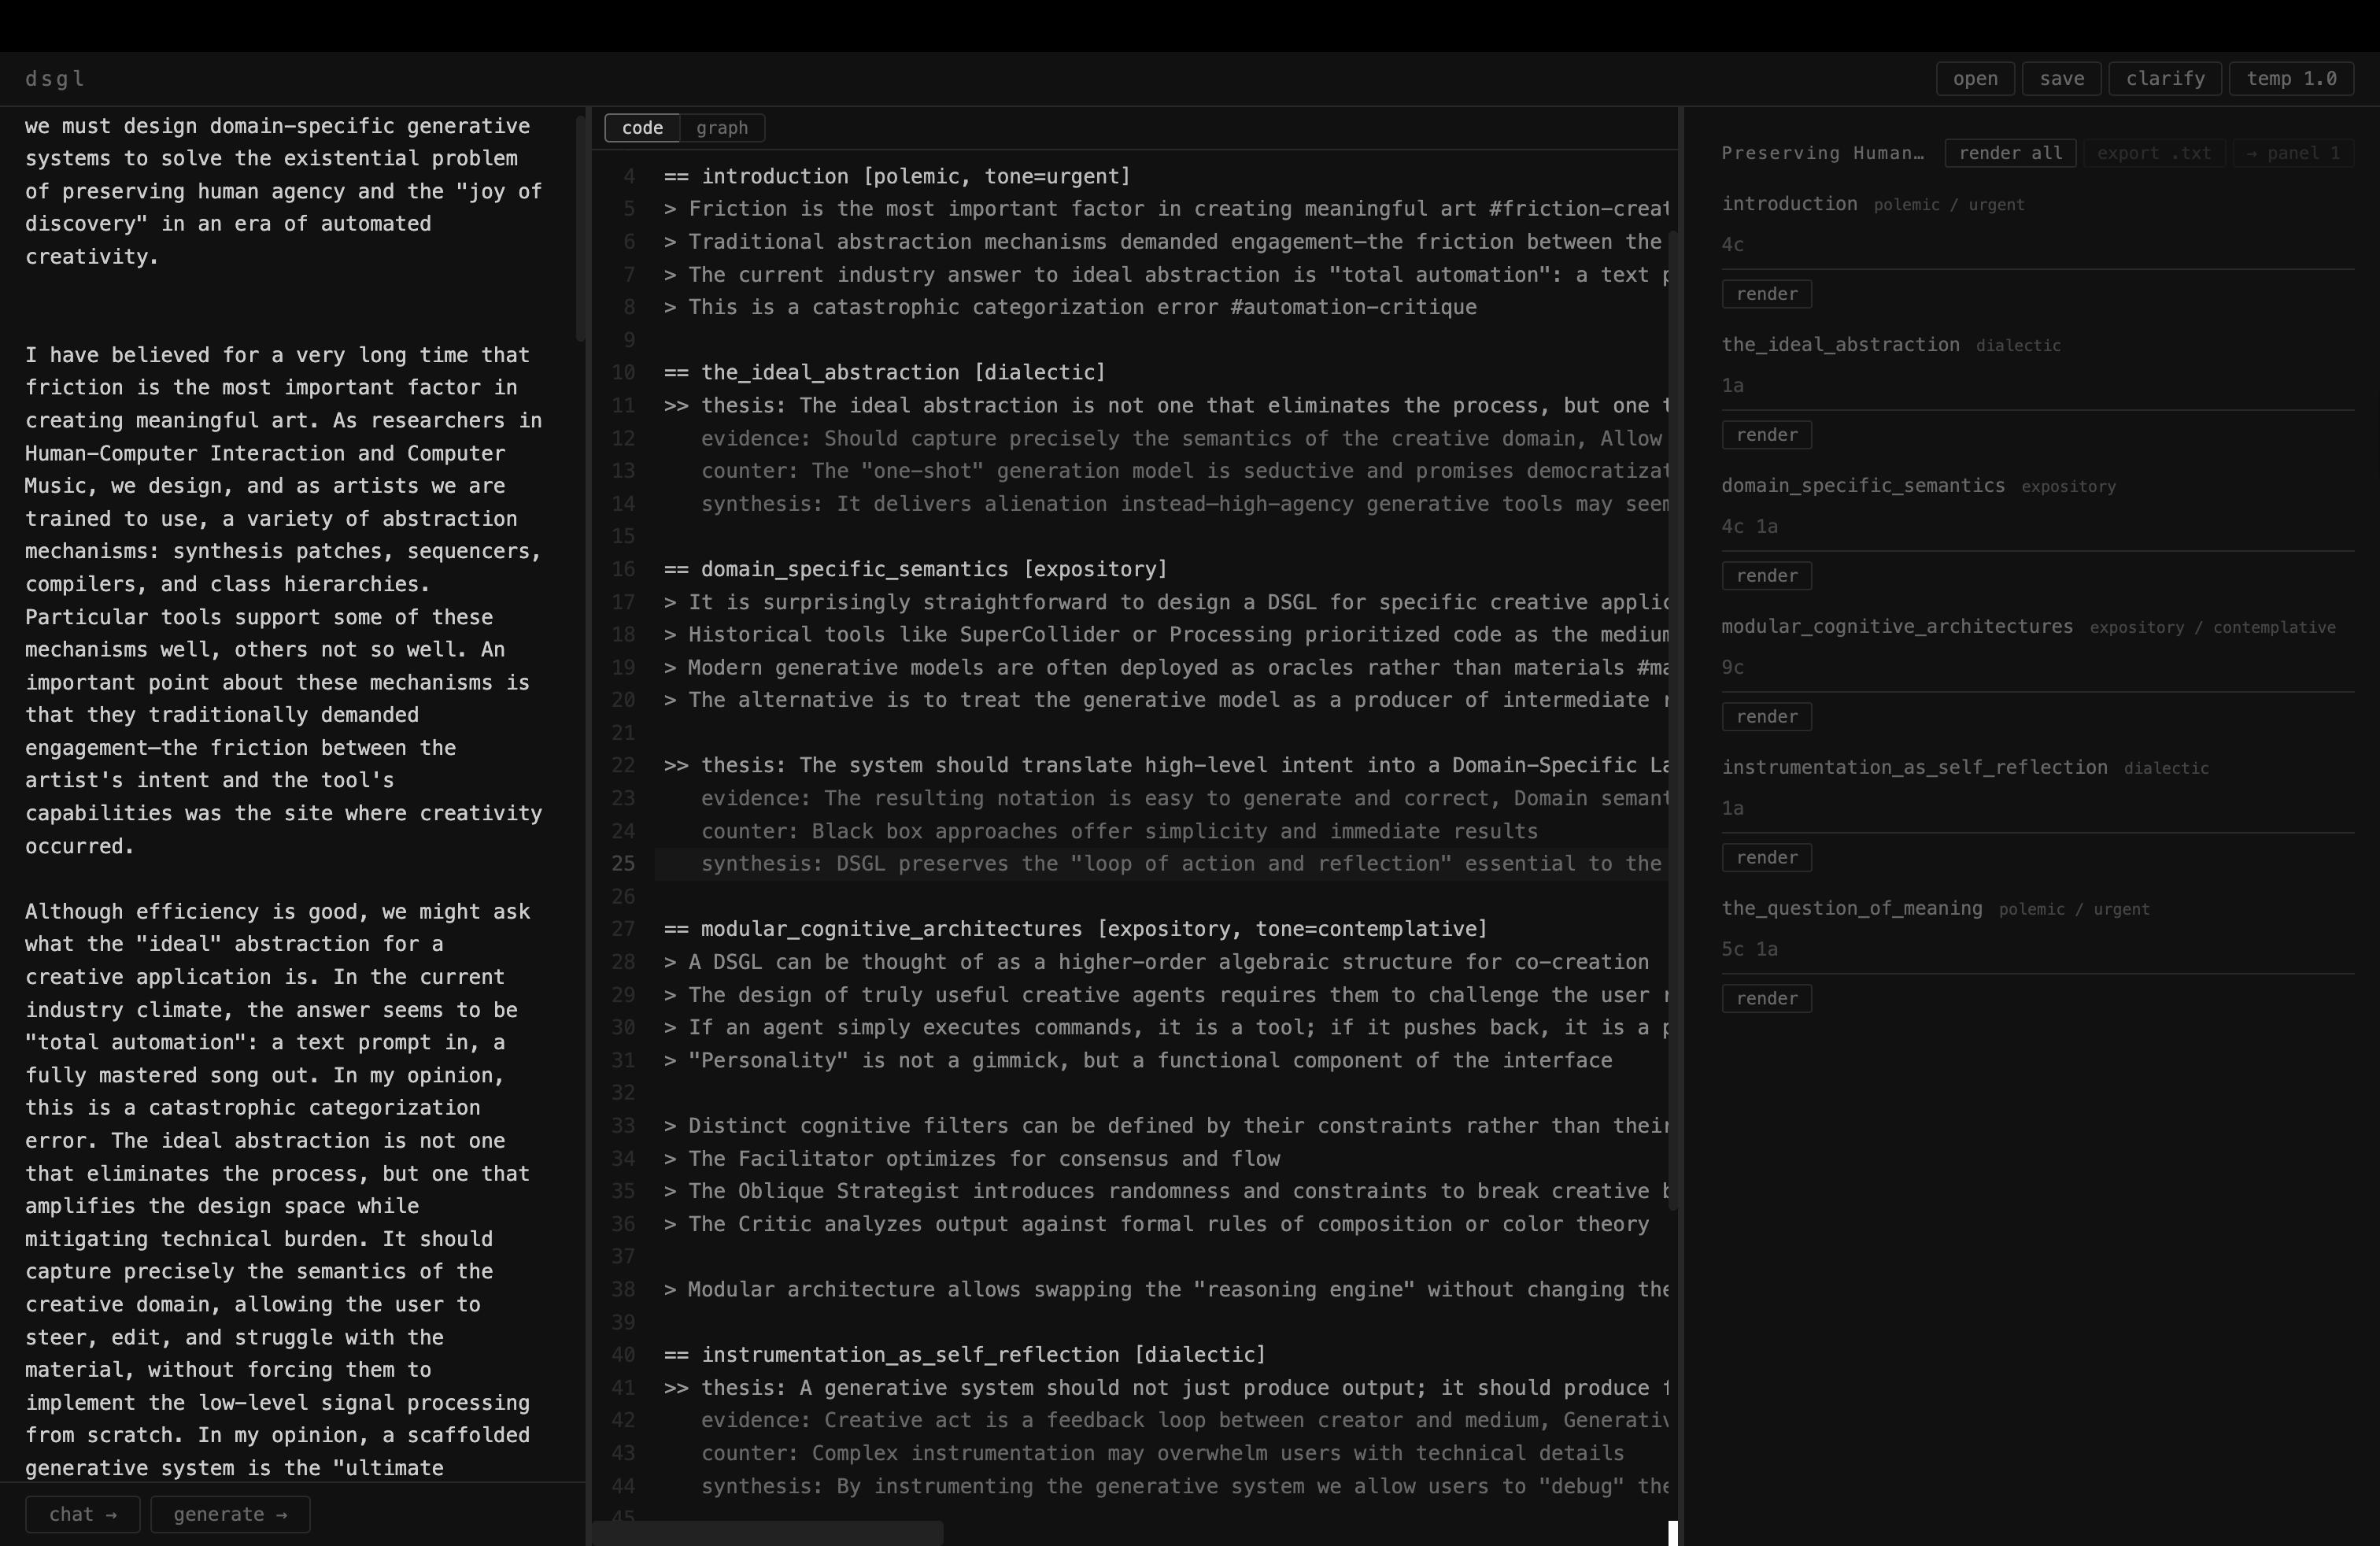
\includegraphics[width=\textwidth]{Interface.png}
  \caption{The interface of Theo, an early prototype of a Domain-Specific Generative Language for essay composition. The three panels correspond to intent (left), structure (center), and artifact (right). The center panel is the intermediate representation that a prompt-based workflow lacks.}
  \label{fig:interface}
\end{figure}

\begin{thebibliography}{10}

\bibitem{iverson1980}
K.~E. Iverson, ``Notation as a Tool of Thought,''
\emph{Communications of the ACM}, vol.~23, no.~8, pp.~444--465, 1980.

\bibitem{hudak1996}
P.~Hudak, ``Building Domain-Specific Embedded Languages,''
\emph{ACM Computing Surveys}, vol.~28, no.~4es, p.~196, 1996.

\bibitem{vercoe1986}
B.~Vercoe, ``Csound: A Manual for the Audio Processing System,''
MIT Media Lab, 1986.

\bibitem{reas2007}
C.~Reas and B.~Fry, \emph{Processing: A Programming Handbook for Visual Designers and Artists}.
MIT Press, 2007.

\end{thebibliography}

\end{document}
